

\section{Predictive Modeling}

Our models for processor configuration prediction are a set of Support Vector Machines (\SVMs)~\cite{vapnik1998statistical}. We use the
Radial basis kernel because it can model both linear and non-linear classification problems. We use the same methodology to learn all
predictors for the target networking environments and optimization goals (i.e., load time, energy consumption, and \EDP).


\subsection{Network Monitoring and Characterization}
\label{sec:networks}
\begin{table}[!t]
\caption{Networking environment settings}
\vspace{-3mm}
\scriptsize
\begin{center}
        \begin{tabular}{lp{2cm}p{2.5cm}c}
        \toprule
        &\textbf{Uplink bandwidth}&\textbf{Downlink bandwidth}&\textbf{Delay}\\
        \midrule
            \rowcolor[gray]{.92}Regular 2G                     &50kbps&100kbps&1000ms\\
            Good 2G                             &150kbps&250kbps&300ms\\
            \rowcolor[gray]{.92}Regular 3G      &300kbps&550kbps&500ms\\
            Good 3G                             &1.5Mbps&5.0Mbps&100ms\\
            \rowcolor[gray]{.92}Regular 4G      &1.0Mbps&2.0Mbps&80ms\\
            Good 4G                             &8.0Mbps&15.0Mbps&50ms\\
            \rowcolor[gray]{.92}WiFi            &15Mbps&30Mbps&5ms\\
        \bottomrule
        \end{tabular}
\end{center}
\label{tab:networkDetails}
\vspace{-5mm}
\end{table}

\begin{figure}[!t]
\begin{center}
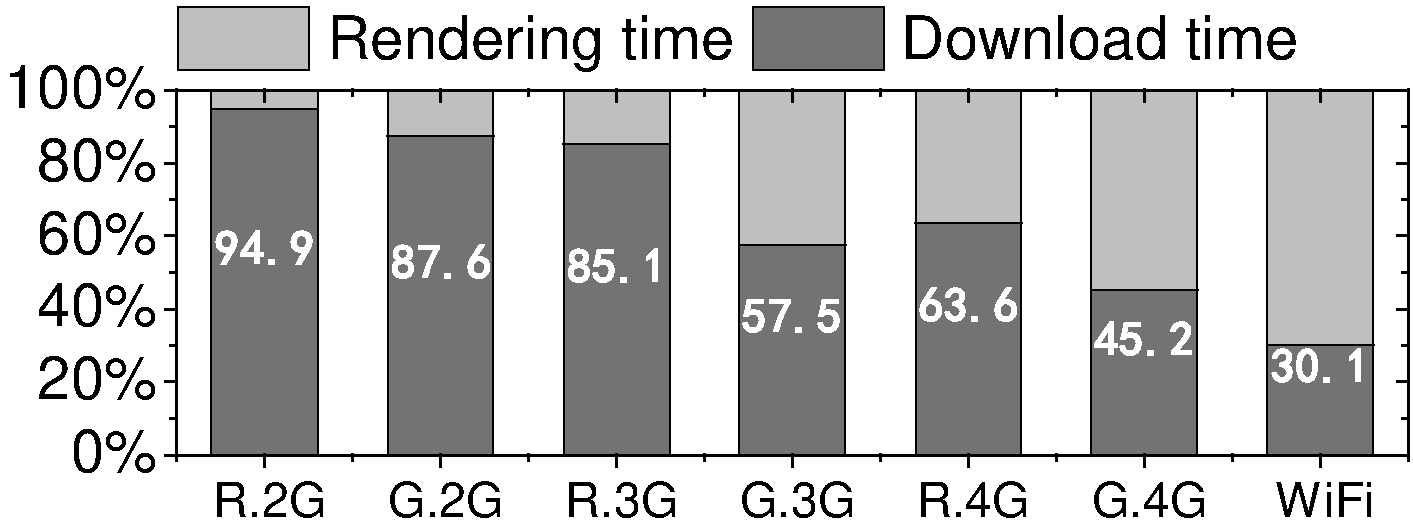
\includegraphics[width=0.45\textwidth]{figure/network.pdf}
\end{center}
\vspace{-2mm}
\caption{Webpage rendering time w.r.t. content download time when using the \Interactive governor.}
\vspace{-4mm}
\label{fig:latency}
\end{figure}


The communication network has a significant impact on the web rendering strategy. 
Table~\ref{tab:networkDetails} lists the networking environments considered in this work. The settings and categorizations are based on the
measurements given by an independent study~\cite{opensignalUK}.  Figure~\ref{fig:latency} shows the webpage rendering time with respect to
the download time under each networking environment when using the \Interactive governor.  The download
time dominates the end to end turnaround time for a 2G and a Regular 3G environments; and by contrast, the rendering time accounts for most
of the turnaround time for a Good 4G and a WiFi environments when the delay is small.


In this work, we learn a predictor per optimization goal for each of the seven networking environments. 
To determine which network environment
the user is currently in, we develop a lightweight network monitor to measure the network bandwidths and delay between the web server and
the device. The network monitor utilizes the communication link statistics that are readily available on commodity smartphones. Measured
data are averaged over the measurement window. The
measurements are then used to map the user's networking environment to one of the pre-defined settings in Table~\ref{tab:networkDetails},
by finding which of the settings is closest to the measured values. The closeness or distance, $d$, is calculated using the following
formula: \vspace{-1mm}
\begin{equation}
d = \alpha |db_{m} - db| + \beta |ub_{m} - ub| + \gamma |d_{m} - d|
\label{eq:cat}
\end{equation}

where $db_m$, $ub_m$, and $d_m$ are the measured downlink bandwidth, upload bandwidth and delay respectively, $db$, $ub$, and $d$ are the
downlink bandwidth, upload bandwidth and delay of a network category, and $\alpha$, $\beta$, $\gamma$ are weights. The weights are
automatically learned from the training data, with an averaged value of 0.3, 0.1 and 0.6 respectively for $\alpha$, $\beta$, and $\gamma$.


\subsection{Training the Predictor}



%\begin{table}[!t]
%\caption{Optimal processor configurations for web rendering under Regular 3G and WiFi network environments}
%\scriptsize
%\begin{center}
%        \begin{tabular}{lccccccccc}
%        \toprule
%        \rowcolor[gray]{.92}& \multicolumn{2}{c}{Load time} &\multicolumn{2}{c}{Energy}& \multicolumn{2}{c}{EDP} \\
%        & A15 & A7 & A15 & A7 & A15 & A7\\
%        \midrule
%             \multirow{4}{*}{Regular 3G}     &\fcolorbox{white}{lightgray}{1.6}&0.4   &0.4&\fcolorbox{white}{lightgray}{0.4}     &\fcolorbox{white}{lightgray}{0.8}&0.4\\
%                            &\fcolorbox{white}{lightgray}{1.7}&0.8   &\fcolorbox{white}{lightgray}{0.4}&0.4     &\fcolorbox{white}{lightgray}{0.8}&0.8\\
%                            &\fcolorbox{white}{lightgray}{1.8}&0.8   &\fcolorbox{white}{lightgray}{0.8}&0.4     &\fcolorbox{white}{lightgray}{0.4}&0.4\\
%                            &\fcolorbox{white}{lightgray}{1.9}&0.8    &0.8&\fcolorbox{white}{lightgray}{0.8}     &-&- \\
%        \midrule
%             \multirow{4}{*}{WiFi}          &\fcolorbox{white}{lightgray}{1.6}&0.4    &\fcolorbox{white}{lightgray}{0.8}&0.4     &\fcolorbox{white}{lightgray}{1.2}&0.8\\
%                            &\fcolorbox{white}{lightgray}{1.7}&0.8   &\fcolorbox{white}{lightgray}{0.8}&0.8     &\fcolorbox{white}{lightgray}{1.2}&0.4\\
%                           &\fcolorbox{white}{lightgray}{1.8}&0.8    &\fcolorbox{white}{lightgray}{1.2}&0.4     &\fcolorbox{white}{lightgray}{0.8}&0.8\\
%                            &\fcolorbox{white}{lightgray}{1.9}&0.8    &-&-                                      &-&-      \\
%        \bottomrule
%        \end{tabular}
%\end{center}
%\label{tab:bestConfig}
%\vspace{-5mm}
%\end{table}

The training process involves finding the best processor configuration and extracting feature values for each training webpage,
and learn a model from the training data.


\cparagraph{Generate Training Data.}
%Our predictor is built \emph{offline} using a set of training webpages.
In this work, we used around 900 webpages to train a \SVM predictor; we then evaluate the learnt model on the other 100 unseen webpages.
These training webpages are selected from the landing page of the top 1000 hottest websites ranked by \texttt{www.alexa.com}. We use Netem~\cite{hemminger2005network}, a Linux-based network enumerator, to emulate
various networking environments to generate the training data. We exhaustively execute the rendering
engine under different processor settings and record the optimal configuration for each optimization goal and each networking environment.
We give each optimal configuration a unique label. For each webpage, we also extract values of a set of selected features.

%For example, Table~\ref{tab:bestConfig} lists the processor configurations for 3G and WiFi network environments, where the gray box indicates
%which core to use to run the rendering process.

\cparagraph{Building The Model.} The feature values together with the labeled processor configuration are supplied to a supervised learning
algorithm~\cite{kotsiantis2007supervised}. The learning algorithm tries to find a correlation from the feature values to the optimal
configuration and produces a \SVM model per networking environment per optimization goal. Because we target two optimization metrics and
seven networking environments, we have constructed 14 \SVM models in total. 

\subsection{Web Features \label{sec:web_features}}
One of the key aspects in building a successful predictor is finding the right features to characterize the input workload. In this work,
we consider a set of features extracted from the web contents. These features are collected by our feature extraction pass. To gather the
feature values, the feature extractor  first obtains a reference for each \DOM element by traversing the \DOM tree and then uses the
Chromium API, \texttt{document.getElementsByID}, to collect node information. We started from 214 raw features, including the number of
\DOM nodes, HTML tags and attributes of different types, and the depth of the \DOM tree, etc. All these features can be collected at
runtime from the browser. The types of the raw features are given in Table~\ref{tab:rawfeature}. These features are selected based
on our intuition and prior work~\cite{ren2016optimise,nejati2016depth,asrese2016wepr}.
It is important to note that the
collected feature values are encoded to a vector of real values.



\begin{figure}[!t]
	\centering
	\subfloat[][Principal components]{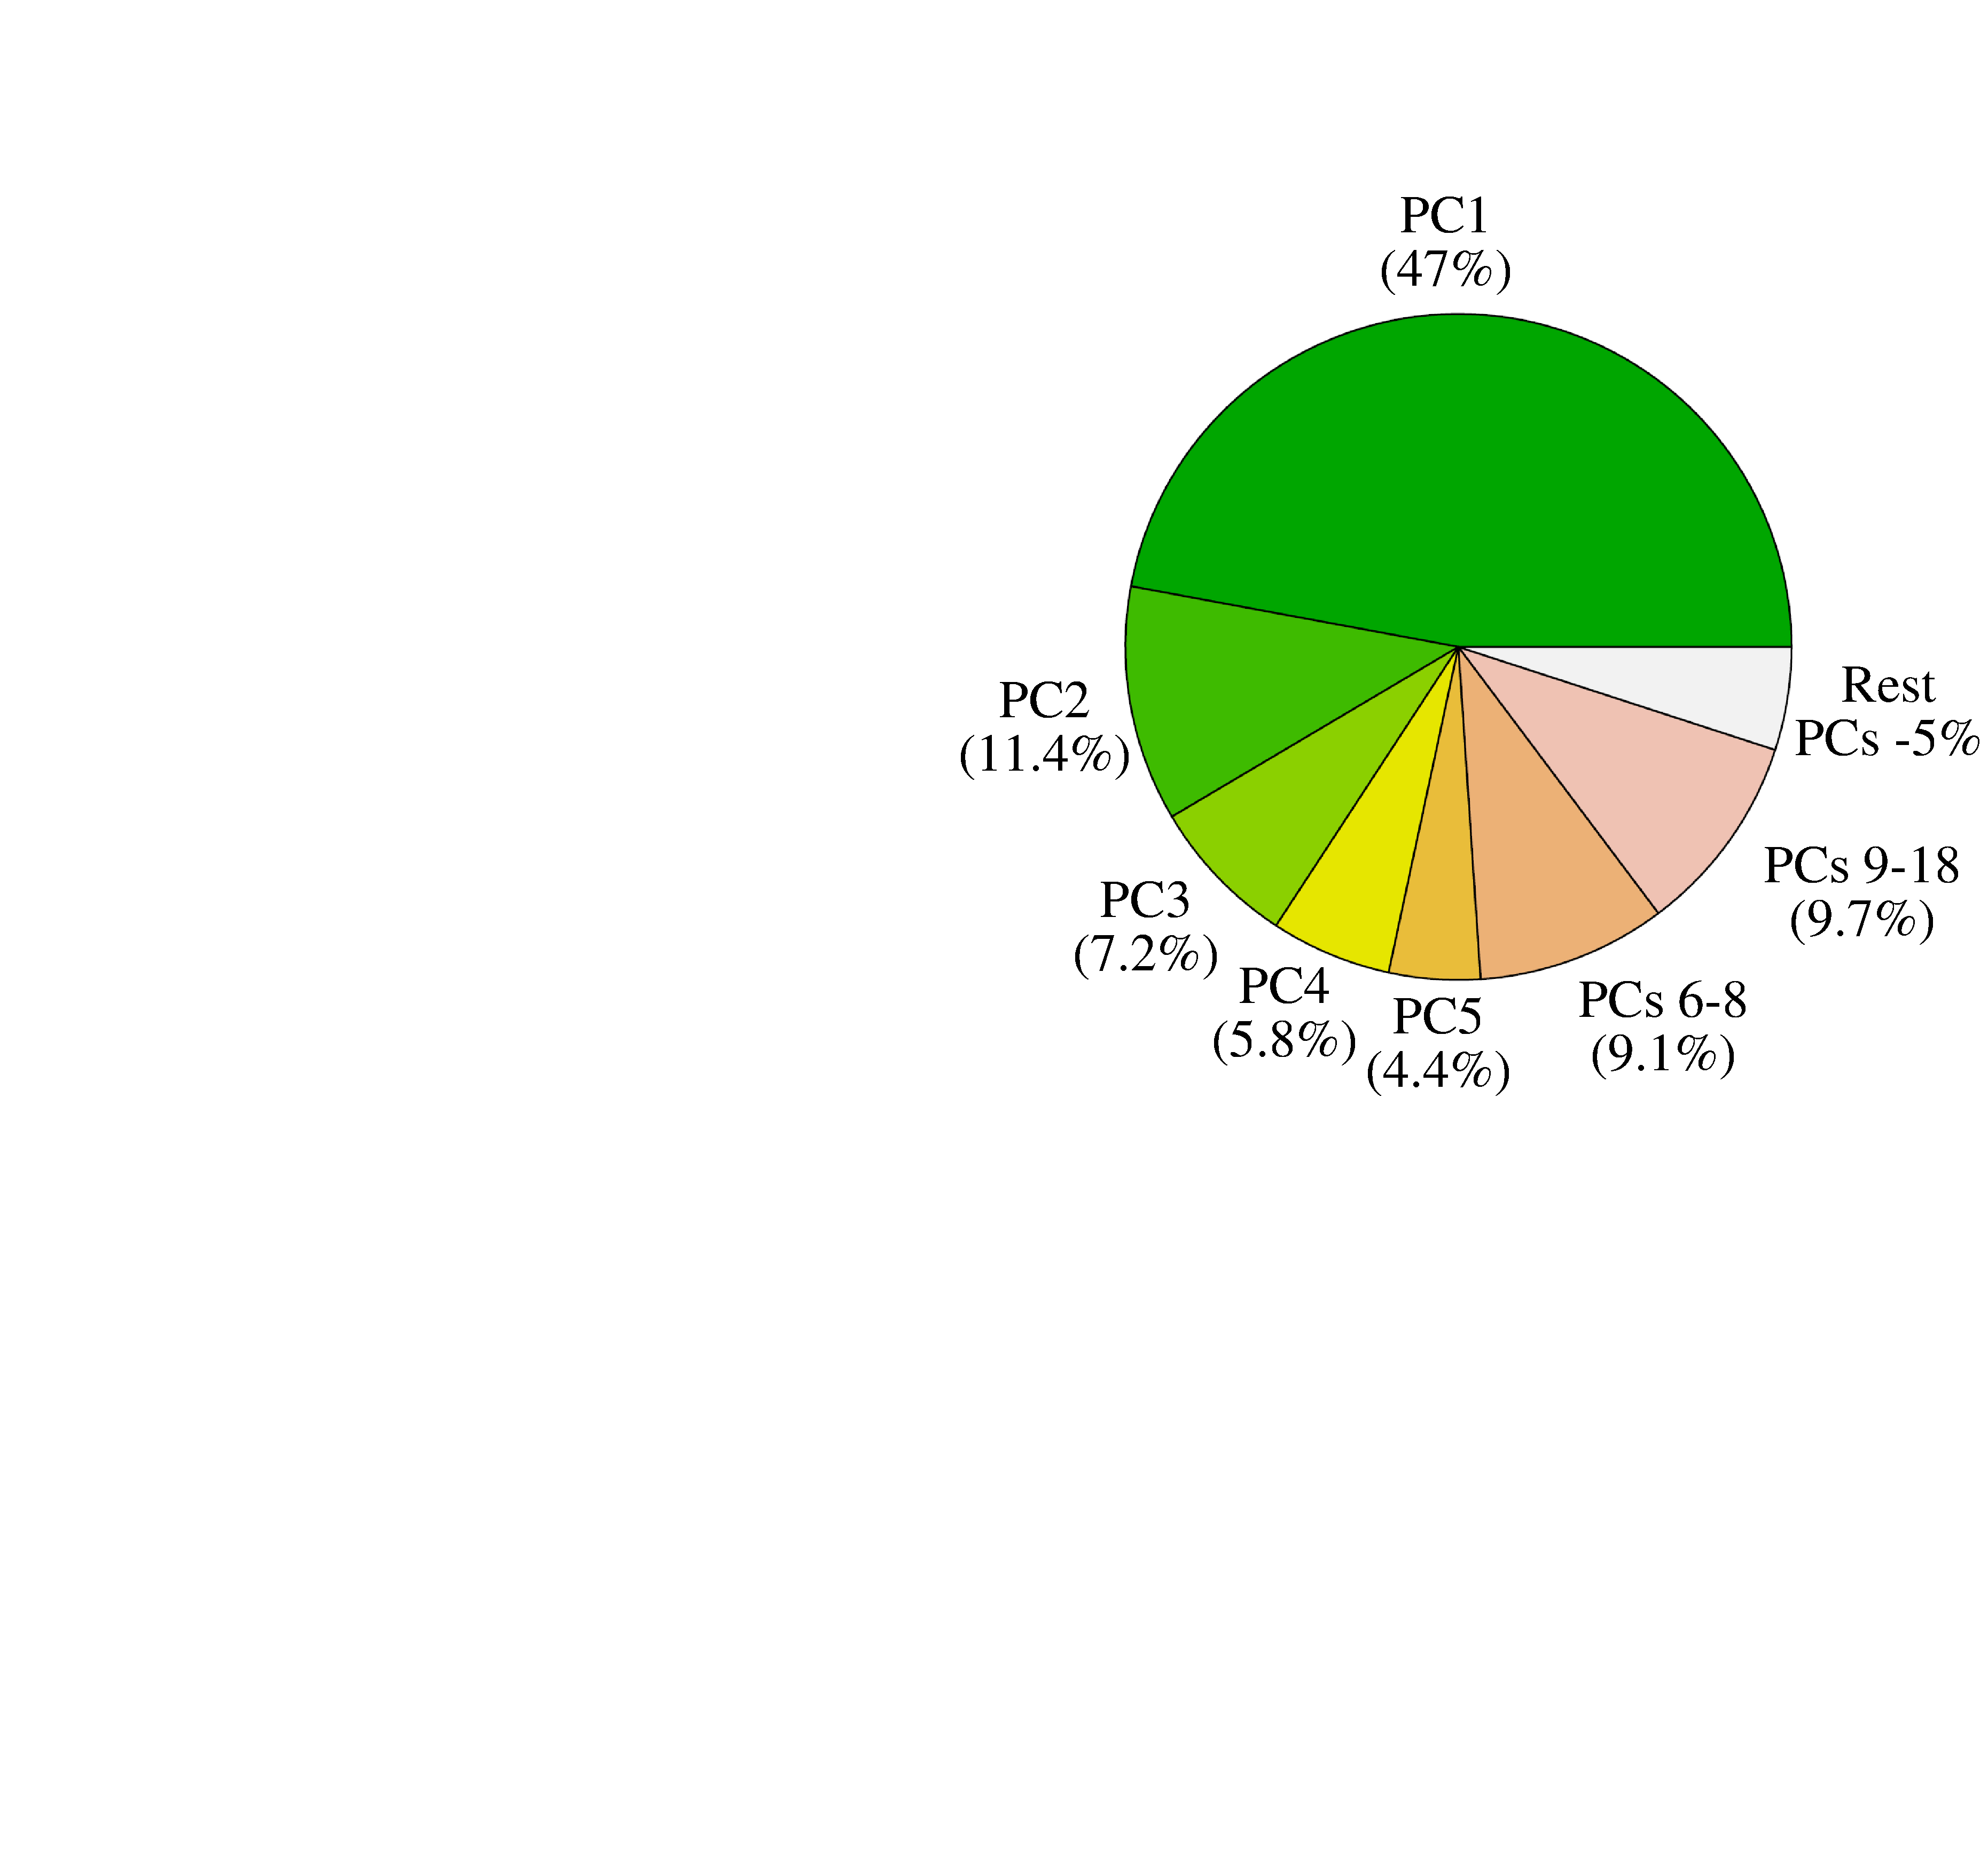
\includegraphics[width=0.23\textwidth]{figure/pca.pdf}}
    \hfill
    \subfloat[][Top 7 most important features]{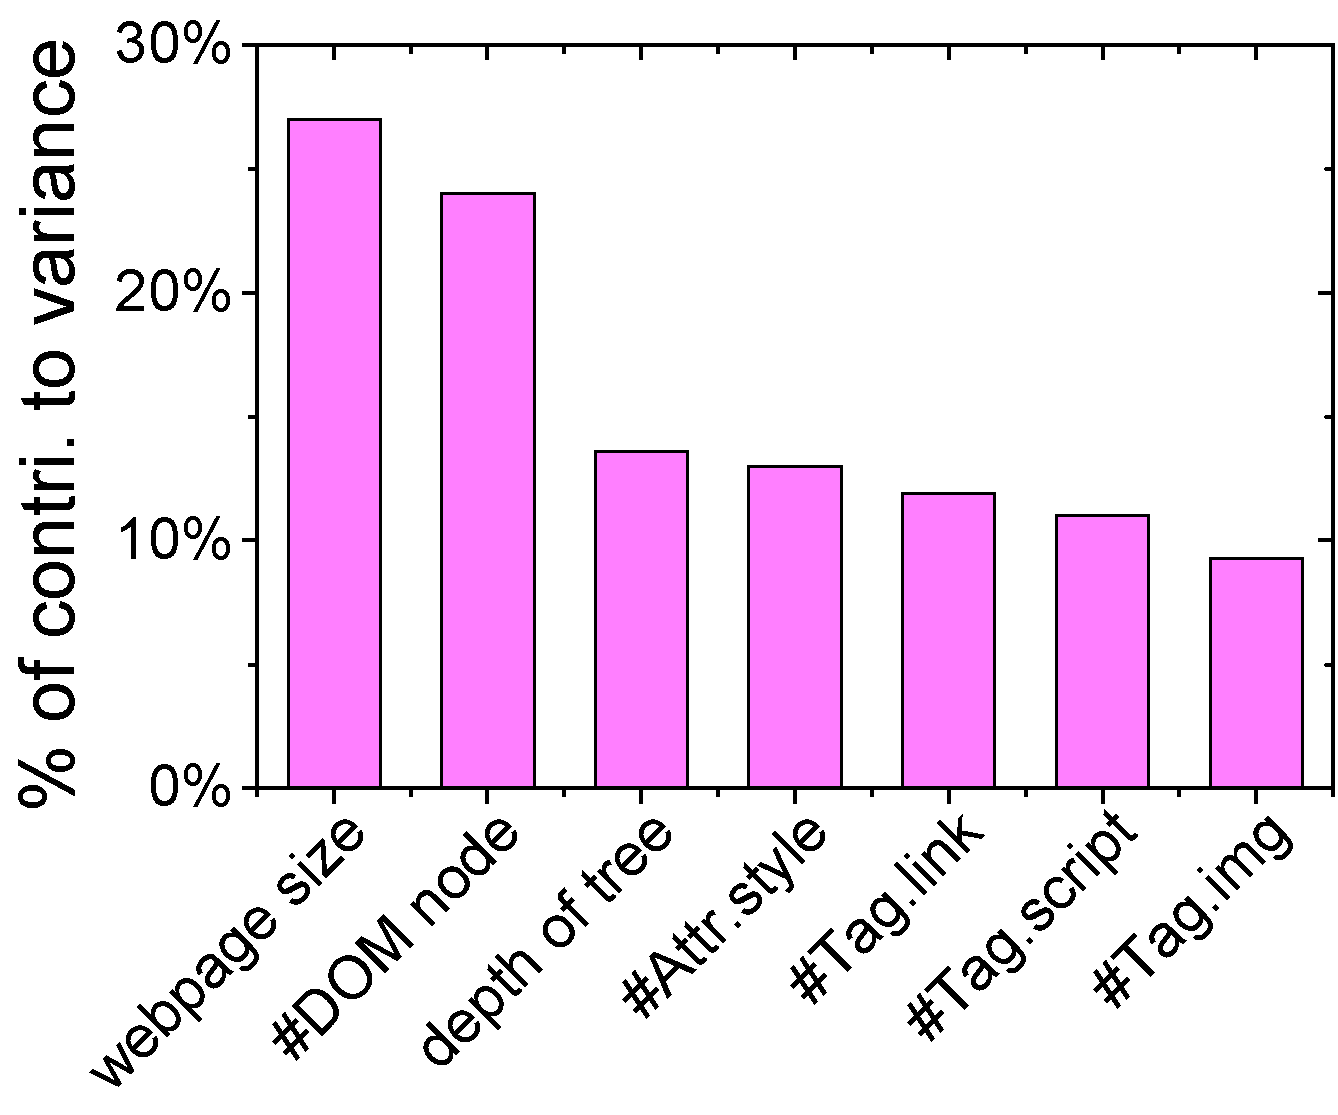
\includegraphics[width=0.23\textwidth]{figure/pcacontri.pdf}}
    \vspace{-2mm}
    \caption{The percentage of principal components (\PCs) to the overall feature variance (a), and contributions of the seven most important
     raw features in the \PCA space (b).}
    \label{fig:pca}
    \vspace{-4mm}
\end{figure}



\cparagraph{Feature Reduction.} To improve the generalization ability of our models, i.e., reducing the likelihood of over-fitting on our training data, we reduce some features
through applying Principal Component Analysis (\PCA)~\cite{dunteman1989principal} to the raw feature
space. \PCA transforms the original inputs into a set of principal components (\PCs) that are linear combinations of the inputs. After
applying \PCA to the 214 raw features, we choose the top 18 principal components (\PCs) which account for around 95\% of the variance of
the original feature space. We record the \PCA transformation matrix and use it to transform the raw features of the new webpage to \PCs
during runtime deployment. Figure ~\ref{fig:pca}a illustrates how much feature variance that each component accounts for. This figure shows
that predictions can accurately draw upon a subset of aggregated feature values.

\cparagraph{Feature Normalization.} Before passing our features to a machine learning model we need to scale each of the features to a
common range (between 0 and 1) in order to prevent the range of any single feature being a factor in its importance. Scaling features does
not affect the distribution or variance of their values. To scale the features of a new webpage during deployment we record the minimum and
maximum values of each feature in the training dataset, and use these to scale the corresponding features.

\cparagraph{Feature Analysis.} To understand the usefulness of each raw feature, we apply the Varimax rotation~\cite{manly2016multivariate}
to the \PCA space. This technique quantifies the contribution of each feature to each \PC. Figure~\ref{fig:pca}b shows the top 7 dominant
features based on their contributions to the \PCs. Features like the webpage size and the number of \DOM nodes are most important,
because they strongly correlate to the download time and the complexity of the webpage. Other features like the depth of the \DOM tree, and
the numbers of different attributes and tags, are also useful, because they determine how the webpage should be presented
and how do they correlate to the rendering cost. 

%Using this technique, we sort the raw features and list top 10 in Table ~\ref{tab:selected_features} according to the importance.

\begin{table}[t!]
\caption{Raw web feature categories}
\vspace{-2mm}
\small
\centering
        \begin{tabular}{rll}
        \toprule
        \multirow{2}{*}{DOM Tree} & \#DOM nodes & depth of tree \\
                & \#each HTML tag & \#each HTML attr. \\
        \rowcolor[gray]{.92}Other  & size of the webpage (Kilobytes) & \\
        \bottomrule
        \end{tabular}
\label{tab:rawfeature}
\vspace{-2mm}
\end{table}

%\begin{table}[!t]
%\caption{Selected web features}
%\small
%\centering
%        \begin{tabular}{rlrl}
%        \toprule
%                            1&size of the webpage    &6&\#Tag.script\\
%        \rowcolor[gray]{.92}2&\#DOM nodes            &7&\#Tag.img  \\
%                            3&depth of tree          &8&\#Attr.content \\
%        \rowcolor[gray]{.92}4&\#Attr.style           &9&\#Tag.img\\
%                           5&\#Tag.link            &10&\#Attr.media \\
%        \bottomrule
%        \end{tabular}
%\label{tab:selected_features}
%\vspace{-2mm}
%\end{table}






%Figure~\ref{fig:example} compares the resultant performance of our model against two widely used CPU frequency governors: \Powersave and
%\Interactive. The x-axis of the diagram shows the load time for the three webpages and the y-axis shows the CPU frequency chosen by each
%scheme. We also give the power consumption of each scheme.


